% Created 2012-05-03 Thu 13:32
\documentclass[11pt]{article}
\usepackage[utf8]{inputenc}
\usepackage[T1]{fontenc}
\usepackage{graphicx}
\usepackage{longtable}
\usepackage{float}
\usepackage{wrapfig}
\usepackage{soul}
\usepackage{amssymb}
\usepackage{hyperref}


\title{SuunnitteluDokumentti}
\author{jarmo}
\date{03 May 2012}

\begin{document}

\maketitle

\setcounter{tocdepth}{3}
\tableofcontents
\vspace*{1cm}
\section{JOHDANTO (1)}
\label{sec-1}

\subsection{Järjestelmän tarkoitus}
\label{sec-1.1}

\begin{itemize}
\item Tiivis kuvaus siitä mistä on kyse.
\item Millaisen toiminnan tukemiseen järjestelmä on tarkoitettu.
\item Mitkä ovat järjestelmän tavoitteet.
\item Nämä tiedot saa yleensä tehtäväkuvauksesta.
\item Järjestelmän käyttötarkoituksena on toteuttaa esimerkiksi kurssikyselyitä, joihin tässä tapauksessa opiskelijat voivat nopeasti vastata,
\end{itemize}
  näin saadaan hyödyllistä tietoa esim. kurssin tehtävien vaikseustasosta.
  Tavoitteena on toteuttaa järjestelmä, jolla voi kyselyitä, joihin vastaamiseen ei mene yli minuuttia.

\subsection{Toimintaympäristö}
\label{sec-1.2}

\begin{itemize}
\item Missä laite ja ohjelmistoympäristössä järjestelmän on tarkoitus toimia.
\end{itemize}
\subsection{Rajaukset}
\label{sec-1.3}

\begin{itemize}
\item Mahdolliset rajaukset koskien määrittelyn, suunnittelun ja toteutuksen laajuutta.
\end{itemize}
\subsubsection{Deploy}
\label{sec-1.3.1}

\begin{itemize}
\item Kaikkialla, missä postgresql tietokanta, ruby 1.9.2-p290 ja rails 3.2.2
\end{itemize}
\subsubsection{Develpoment}
\label{sec-1.3.2}

\begin{itemize}
\item Kaikkialla, missä sqlite3 asennettuna, ruby 1.9.2-p290 ja rails 3.2.2
\end{itemize}
\subsection{Toteutusympäristö}
\label{sec-1.4}

\subsection{Missä ympäristössä työ toteutetaan.}
\label{sec-1.5}

\begin{itemize}
\item Ruby on rails kielellä ja deployaus herokuun.
\end{itemize}
\section{Yleiskuva järjestelmästä (2)}
\label{sec-2}

\subsection{Sidosryhmäkaavio}
\label{sec-2.1}

   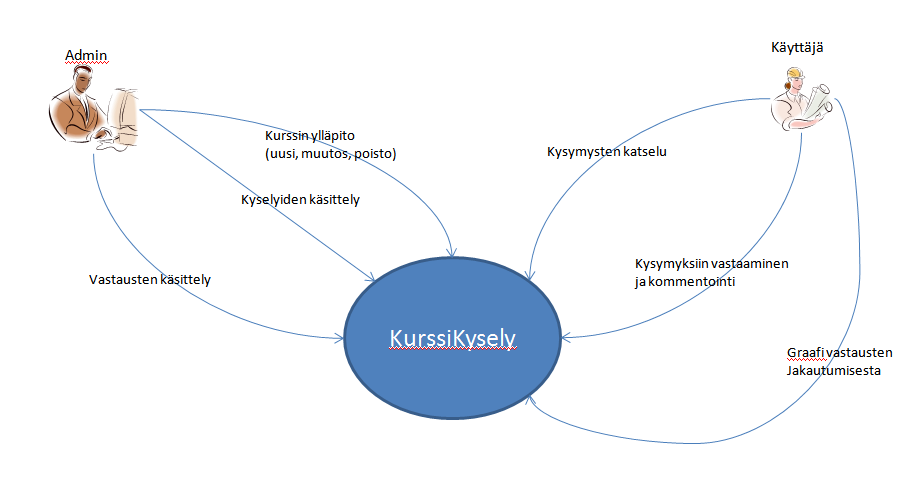
\includegraphics[width=10em]{sidosryhmakaavio.png}
\subsection{Käyttäjäruhmät}
\label{sec-2.2}

\begin{itemize}
\item Kursilainen (ei autentikointia) tarkoitetaan kurssilaista, jolle ehdotetaan kyselyyn vastaamista.
\item Admin on henkilö, jolla oikeudet luoda uusia kursseja ja kysymyksiä, sekä lukea kommentteja
\end{itemize}
\section{Käyttätapaukset (3)}
\label{sec-3}

   Pääsivulla / cources -sivulla
   Admin
   On kaikista kursseista listaus
\begin{itemize}
\item Voi luoda uuden kurssin
\item voi poistaa kurssin
\item voi siirtyä katselemaan kursseja
\end{itemize}
   Kurssin sivulla / cources/:id
   Admin
\begin{itemize}
\item Näkee kaikki kyselyt
\item Voi luoa uusia kyselyitä
\item Voi poistaa kyselyitä, esim. jos kysymyksessä on virheitä
\item Merkkaa mihin kysymyksiin vastaaminen mahdollista
\end{itemize}
   Peruskäyttäjä/Anonyymi
\begin{itemize}
\item Näkee kysymykset, joihin vastaaminen mahdollista
\end{itemize}
   Kysymyssivulla / cources/:id/:kysID
   Admin
\begin{itemize}
\item Näkee vastaukset
\item Voi vastata kysymykseen
\item Näkee vastauksen jälkeen jonkinasteisen graafin vastausten jakautumisesta
\item Näkee kysymykseen liittyvät kommentit
\end{itemize}
   Peruskäyttäjä/Anonyymi
\begin{itemize}
\item Voi vastata kysymykseen
\item Voi kommentoida kysymystä
\item Näkee vastauksen jälkeen jonkinasteisen graafin vastausten jakautumisesta
\end{itemize}
\section{Järjestelmän tietosisältö (4)}
\label{sec-4}

  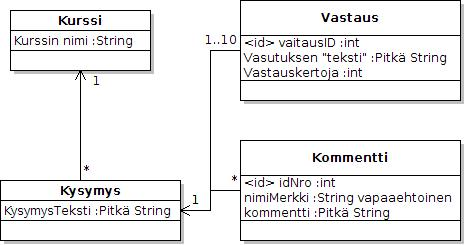
\includegraphics[width=10em]{tietosisalto.jpeg}
\section{Käyttöliittymän hahmotelma (5)}
\label{sec-5}

   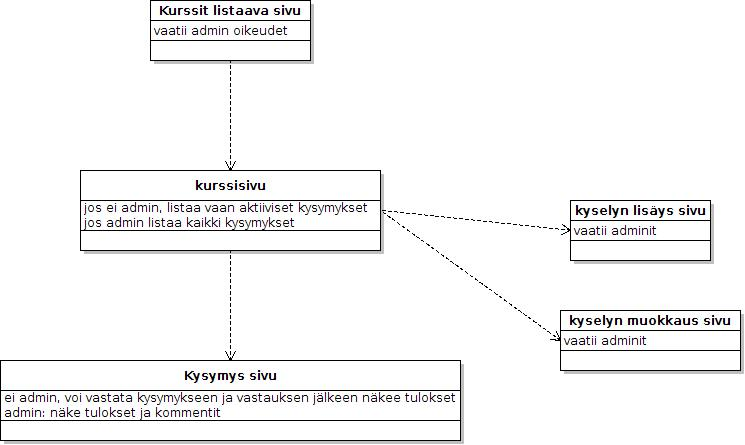
\includegraphics[width=10em]{sivukaavio.jpeg}
\section{Relaatiotietokantakaavio (6)}
\label{sec-6}

    \href{file:///home/jarmo/aktivatorPlus/docs/tietokanta1.gif}{file:tietokanta1.gif}


\end{document}
